\begin{task}
\TT{Wyznacz współczynniki zespolonego szeregu Fouriera dla okresowego sygnału $f(t)$ przedstawionego na rysunku. Narysuj widmo amplitudowe i fazowe sygnału.}{Calculate coefficients of the periodic signal $f(t)$ shown below for the expansion into a complex exponential Fourier series. Draw magnitude and phase spectra.} 

\begin{figure}[H]
\centering
\begin{tikzpicture}
  %\draw (0,0) circle (1in);
  \draw[->] (-3.0,+0.0) -- (+5.0,+0.0) node[right] {$t$};
  \draw[->] (+0.0,-1.5) -- (+0.0,+2.0) node[above] {$f(t)$};
  \draw[scale=1.0,domain=-1.5:-1.0,samples=100,smooth,variable=\x,red,thick] plot ({\x},{0.0+1*cos(\x*180.0/3.141592*1*3.141592/1.0)});
  \draw[-,red, thick] (-1.0,-1.0) -- (-1.0,0.0) -- (0.0,0.0) -- (0.0,1.0);
  \draw[scale=1.0,domain=0.0:1.0,samples=100,smooth,variable=\x,red,thick] plot ({\x},{0.0+1*cos(\x*180.0/3.141592*1*3.141592/1.0)});
  \draw[-,red, thick] (1.0, -1.0) -- (1.0,0.0) -- (2.0,0.0) -- (2.0,1.0);
  \draw[scale=1.0,domain=2.0:3.0,samples=100,smooth,variable=\x,red,thick] plot ({\x},{0.0+1*cos(\x*180.0/3.141592*1*3.141592/1.0)});
  \draw[-,red, thick] (3.0,-1.0) -- (3.0,0.0) -- (3.5,0.0);
  \draw[-,red, dashed] (-2.0,1.0) -- (4.0,1.0);
  \draw[-,red, dashed] (-2.0,-1.0) -- (4.0,-1.0);
  %\draw[-] (-1.0-0.1,-0.1)--(-1.0+0.1,0.1) node[midway, below, outer sep=10pt,align=center] {$-\frac{T}{2}$};
  \draw[-] (-1.0-0.1,-0.1)--(-1.0+0.1,0.1) node[midway, below, outer sep=5pt] {$-\frac{T}{2}$};
  \draw[-] (+1.0-0.1,-0.1)--(+1.0+0.1,0.1) node[midway, below, outer sep=5pt] {$\frac{T}{2}$};
  \draw[-] (+2.0-0.1,-0.1)--(+2.0+0.1,0.1) node[midway, below, outer sep=5pt] {$T$};
  \draw[-] (-0.1,+1.0-0.1)--(+0.1,+1.0+0.1) node[midway, left] {$A$};
  \draw[-] (-0.1,-1.0-0.1)--(+0.1,-1.0+0.1) node[midway, left] {$-A$};

\end{tikzpicture}
\end{figure}

\TT{W pierwszej kolejności należy opisać sygnał za pomocą wzoru.}{Periodic signal $f(t)$, as a piecewise function, is given by:}

\begin{equation}
f(x)=\begin{cases}A \cdot cos\left( \frac{2\pi}{T} \cdot t\right) & t \in \left ( 0+k \cdot T; \frac{T}{2}+k \cdot T \right ) \\
0 & t \in \left ( \frac{T}{2}+k \cdot T; T+k \cdot T \right )\end{cases} \wedge k \in \TT{C}{Z}
\end{equation}

\TT{Współczynnik $F_0$ wyznaczamy ze wzoru:}{The $F_0$ coefficient is defined as:}

\begin{equation}
F_0=\frac{1}{T}\int_{T}f(t) \cdot dt
\end{equation}

\TT{Podstawiamy do wzoru wzór naszej funkcji w pierwszym okresie $k=0$}{For the period $t \in (0; T)$, i.e. $k=0$, we get:}

\begin{align*}
F_0&=\frac{1}{T}\int_{T}f(t) \cdot dt=\\
&=\frac{1}{T}\left(\int_{0}^{\frac{T}{2}} A \cdot cos\left( \frac{2\pi}{T} \cdot t\right) \cdot dt + \int_{\frac{T}{2}}^{T} 0 \cdot dt\right)=\\
&=\frac{1}{T}\left(A \cdot \int_{0}^{\frac{T}{2}} cos\left( \frac{2\pi}{T} \cdot t\right) \cdot dt + 0\right)=\\
&=\frac{A}{T} \cdot \int_{0}^{\frac{T}{2}} cos\left( \frac{2\pi}{T} \cdot t\right) \cdot dt =\\
&=\begin{Bmatrix}
z&=\frac{2\pi}{T} \cdot t\\
dz&=\frac{2\pi}{T} \cdot dt\\
dt&=\frac{1}{\frac{2\pi}{T}} \cdot dz\\
dt&=\frac{T}{2\pi} \cdot dz\\
\end{Bmatrix}=\\
&=\frac{A}{T} \cdot \int_{0}^{\frac{T}{2}} cos\left(z\right) \cdot \frac{T}{2\pi} \cdot dz =\\
&=\frac{A}{T} \cdot \frac{T}{2\pi} \cdot \int_{0}^{\frac{T}{2}} cos\left(z\right)  \cdot dz =\\
&=\frac{A}{T} \cdot \frac{T}{2\pi} \cdot \left. sin\left(z\right)  \right|_{0}^{\frac{T}{2}} =\\
&=\frac{A}{2\pi} \cdot \left. sin\left(\frac{2\pi}{T} \cdot t\right)  \right|_{0}^{\frac{T}{2}} =\\
&=\frac{A}{2\pi} \cdot \left( sin\left(\frac{2\pi}{T} \cdot \frac{T}{2}\right) - sin\left(\frac{2\pi}{T} \cdot 0\right) \right) =\\
&=\frac{A}{2\pi} \cdot \left( sin\left(pi\right) - sin\left(0\right) \right) =\\
&=\frac{A}{2\pi} \cdot \left( 0 -0 \right) =\\
&=\frac{A}{2\pi} \cdot 0 =\\
&=0 
\end{align*}

\TT{Wartość współczynnika $F_0$ wynosi $0$.}{The $F_0$ coefficient equals $0$.}


\TT{Współczynniki $F_k$ wyznaczamy ze wzoru:}{The $F_k$ coefficients are defined as:}


\begin{equation}
F_k=\frac{1}{T}\int_{T}f(t) \cdot e^{- \jmath \cdot k \cdot \frac{2\pi}{T} \cdot t} \cdot dt
\end{equation}

\TT{Podstawiamy do wzoru wzór naszej funkcji w pierwszym okresie $k=0$}{For the period $t \in (0; T)$, i.e. $k=0$, we get:}

\begin{align*}
F_k&=\frac{1}{T}\int_{T}f(t) \cdot e^{-\jmath \cdot k \cdot \frac{2\pi}{T} \cdot t} \cdot dt=\\
&=\frac{1}{T}\left( \int_{0}^{\frac{T}{2}}A \cdot cos\left( \frac{2\pi}{T} \cdot t\right) \cdot e^{ - \jmath \cdot k \cdot \frac{2\pi}{T} \cdot t} \cdot dt + \int_{\frac{T}{2}}^{T} 0 \cdot e^{ - \jmath \cdot k \cdot \frac{2\pi}{T} \cdot t} \cdot dt\right)=\\
&=\frac{1}{T}\left( A \cdot  \int_{0}^{\frac{T}{2}}cos\left( \frac{2\pi}{T} \cdot t\right) \cdot e^{ -\jmath \cdot k \cdot \frac{2\pi}{T} \cdot t} \cdot dt + \int_{\frac{T}{2}}^{T} 0 \cdot dt\right)=\\
&=\begin{Bmatrix}
cos\left(x\right) = \frac{e^{\jmath \cdot x}+e^{-\jmath \cdot x}}{2}
\end{Bmatrix}=\\
&=\frac{1}{T}\left( A \cdot  \int_{0}^{\frac{T}{2}} \frac{e^{\jmath \cdot \frac{2\pi}{T} \cdot t}+e^{-\jmath \cdot \frac{2\pi}{T} \cdot t}}{2} \cdot e^{ - \jmath \cdot k \cdot \frac{2\pi}{T} \cdot t} \cdot dt + 0\right)=\\
&=\frac{A}{2\cdot T}\cdot  \int_{0}^{\frac{T}{2}} \left(e^{\jmath \cdot \frac{2\pi}{T} \cdot t}+e^{-\jmath \cdot \frac{2\pi}{T} \cdot t}\right) \cdot e^{- \jmath \cdot k \cdot \frac{2\pi}{T} \cdot t} \cdot dt =\\
&=\frac{A}{2\cdot T}\cdot  \int_{0}^{\frac{T}{2}} \left(e^{\jmath \cdot \frac{2\pi}{T} \cdot t - \jmath \cdot k \cdot \frac{2\pi}{T} \cdot t}+e^{-\jmath \cdot \frac{2\pi}{T} \cdot t - \jmath \cdot k \cdot \frac{2\pi}{T} \cdot t}\right) \cdot dt =\\
&=\frac{A}{2\cdot T}\cdot  \int_{0}^{\frac{T}{2}} \left(e^{\jmath \cdot \frac{2\pi}{T} \cdot \left(1 -k\right) \cdot t}+e^{-\jmath \cdot \frac{2\pi}{T} \cdot \left(1+k\right)\cdot t }\right) \cdot dt =\\
&=\frac{A}{2\cdot T}\cdot \left( \int_{0}^{\frac{T}{2}} e^{\jmath \cdot \frac{2\pi}{T} \cdot \left(1 -k\right) \cdot t} \cdot dt + \int_{0}^{\frac{T}{2}} e^{-\jmath \cdot \frac{2\pi}{T} \cdot \left(1+k\right)\cdot t } \cdot dt \right)=\\
&=\begin{Bmatrix}
z_1=\jmath \cdot \frac{2\pi}{T} \cdot \left(1 -k\right) \cdot t & z_2=-\jmath \cdot \frac{2\pi}{T} \cdot \left(1+k\right)\cdot t\\
dz_1=\jmath \cdot \frac{2\pi}{T} \cdot \left(1 -k\right) \cdot dt & dz_2=-\jmath \cdot \frac{2\pi}{T} \cdot \left(1+k\right)\cdot dt\\
dt=\frac{1}{\jmath \cdot \frac{2\pi}{T} \cdot \left(1 -k\right)} \cdot dz_1 & dt=\frac{1}{-\jmath \cdot \frac{2\pi}{T} \cdot \left(1+k\right)}\cdot dz_2\\
\end{Bmatrix}=\\
&=\frac{A}{2\cdot T}\cdot \left( \int_{0}^{\frac{T}{2}} e^{z_1} \cdot \frac{1}{\jmath \cdot \frac{2\pi}{T} \cdot \left(1 -k\right)} \cdot dz_1 + \int_{0}^{\frac{T}{2}} e^{z_2 } \cdot \frac{1}{-\jmath \cdot \frac{2\pi}{T} \cdot \left(1+k\right)}\cdot dz_2 \right)=\\
&=\frac{A}{2\cdot T}\cdot \left( \frac{1}{\jmath \cdot \frac{2\pi}{T} \cdot \left(1 -k\right)} \cdot \int_{0}^{\frac{T}{2}} e^{z_1} \cdot dz_1 + \frac{1}{-\jmath \cdot \frac{2\pi}{T} \cdot \left(1+k\right)}\cdot \int_{0}^{\frac{T}{2}} e^{z_2 } \cdot dz_2 \right)=\\
&=\frac{A}{2\cdot T}\cdot \left( \frac{T}{\jmath \cdot 2\pi \cdot \left(1 -k\right)} \cdot \int_{0}^{\frac{T}{2}} e^{z_1} \cdot dz_1 - \frac{T}{\jmath \cdot 2\pi \cdot \left(1+k\right)}\cdot \int_{0}^{\frac{T}{2}} e^{z_2 } \cdot dz_2 \right)=\\
&=\frac{A}{2\cdot T}\cdot \frac{T}{\jmath \cdot 2\pi} \cdot \left( \frac{1}{\left(1 -k\right)} \cdot \int_{0}^{\frac{T}{2}} e^{z_1} \cdot dz_1 - \frac{1}{ \left(1+k\right)}\cdot \int_{0}^{\frac{T}{2}} e^{z_2 } \cdot dz_2 \right)=\\
&=\frac{A}{\jmath \cdot 4\pi} \cdot \left( \frac{1}{\left(1 -k\right)} \cdot \left. e^{z_1} \right|_{0}^{\frac{T}{2}} - \frac{1}{ \left(1+k\right)}\cdot \left. e^{z_2 } \right|_{0}^{\frac{T}{2}} \right)=\\
&=\frac{A}{\jmath \cdot 4\pi} \cdot \left( \frac{1}{\left(1 -k\right)} \cdot \left. e^{\jmath \cdot \frac{2\pi}{T} \cdot \left(1 -k\right) \cdot t} \right|_{0}^{\frac{T}{2}} - \frac{1}{ \left(1+k\right)}\cdot \left. e^{-\jmath \cdot \frac{2\pi}{T} \cdot \left(1+k\right)\cdot t } \right|_{0}^{\frac{T}{2}} \right)=\\
&=\frac{A}{\jmath \cdot 4\pi} \cdot \left( \frac{1}{\left(1 -k\right)} \cdot \left(e^{\jmath \cdot \frac{2\pi}{T} \cdot \left(1 -k\right) \cdot \frac{T}{2}} -e^{\jmath \cdot \frac{2\pi}{T} \cdot \left(1 -k\right) \cdot 0}\right) - \frac{1}{ \left(1+k\right)}\cdot \left( e^{-\jmath \cdot \frac{2\pi}{T} \cdot \left(1+k\right)\cdot \frac{T}{2} } - e^{-\jmath \cdot \frac{2\pi}{T} \cdot \left(1+k\right)\cdot 0 }\right) \right)=\\
&=\frac{A}{\jmath \cdot 4\pi} \cdot \left( \frac{1}{\left(1 -k\right)} \cdot \left(e^{\jmath \cdot \pi \cdot \left(1 -k\right) } -e^{0}\right) - \frac{1}{ \left(1+k\right)}\cdot \left( e^{-\jmath \cdot \pi \cdot \left(1+k\right) } - 1\right) \right)=\\
&=\frac{A}{\jmath \cdot 4\pi} \cdot \left( \frac{1}{\left(1 -k\right)} \cdot \left(e^{\jmath \cdot \pi } \cdot e^{-\jmath \cdot k \cdot \pi}  -1\right) - \frac{1}{ \left(1+k\right)}\cdot \left( e^{-\jmath \cdot \pi } \cdot e^{-\jmath \cdot k \cdot \pi } - 1\right) \right)=\\
&=\frac{A}{\jmath \cdot 4\pi} \cdot \left( \frac{1}{\left(1 -k\right)} \cdot \left(-1 \cdot e^{-\jmath \cdot k \cdot \pi}  -1\right) - \frac{1}{ \left(1+k\right)}\cdot \left( -1 \cdot e^{-\jmath \cdot k \cdot \pi } - 1\right) \right)=\\
&=\frac{A}{\jmath \cdot 4\pi} \cdot \left( \frac{1}{\left(1 -k\right)} \cdot \left(- \cdot e^{-\jmath \cdot k \cdot \pi}  -1\right) - \frac{1}{ \left(1+k\right)}\cdot \left( - \cdot e^{-\jmath \cdot k \cdot \pi } - 1\right) \right)=\\
&=\frac{A}{\jmath \cdot 4\pi} \cdot \left( \frac{\left(- e^{-\jmath \cdot k \cdot \pi}  -1\right) \cdot \left(1+k\right) }{\left(1 -k\right) \cdot \left(1+k\right)} - \frac{\left( - e^{-\jmath \cdot k \cdot \pi } - 1\right)  \cdot \left(1 -k\right)}{\left(1 -k\right) \cdot \left(1+k\right)} \right)=\\
&=\frac{A}{\jmath \cdot 4\pi} \cdot \left( \frac{- \cdot e^{-\jmath \cdot k \cdot \pi}  -1 - k \cdot e^{-\jmath \cdot k \cdot \pi}  -k }{\left(1 -k\right) \cdot \left(1+k\right)} - \frac{ - \cdot e^{-\jmath \cdot k \cdot \pi } - 1 +k \cdot e^{-\jmath \cdot k \cdot \pi } +k }{\left(1 -k\right) \cdot \left(1+k\right)} \right)=\\
&=\frac{A}{\jmath \cdot 4\pi} \cdot \left( \frac{- \cdot e^{-\jmath \cdot k \cdot \pi}  -1 - k \cdot e^{-\jmath \cdot k \cdot \pi}  -k + e^{-\jmath \cdot k \cdot \pi } + 1 -k \cdot e^{-\jmath \cdot k \cdot \pi } -k }{1 -k^2} \right)=\\
&=\frac{A}{\jmath \cdot 4\pi} \cdot \left( \frac{ - 2\cdot k \cdot e^{-\jmath \cdot k \cdot \pi}  -2\cdot k}{1 -k^2} \right)=\\
&=-\frac{A \cdot k}{\jmath \cdot 2\pi} \cdot \left( \frac{ e^{-\jmath \cdot k \cdot \pi}  + 1}{1 -k^2} \right)\\
&=\jmath \cdot \frac{A \cdot k}{2\pi} \cdot \left( \frac{ (-1)^{k}  + 1}{1 -k^2} \right)
\end{align*}

\TT{Wartość współczynnika $F_k$ wynosi $\jmath \cdot \frac{A \cdot k}{2\pi} \cdot \left( \frac{ (-1)^{k}  + 1}{1 -k^2} \right)$.}{The $F_k$ coefficients equal to $\jmath \cdot \frac{A \cdot k}{2\pi} \cdot \left( \frac{ (-1)^{k}  + 1}{1 -k^2} \right)$.}

\TT{Współczynnik $F_k$ dla $k=1$ musimy wyznaczyć raz jeszcze, tak więc wyznaczmy go wprost z definicji $F_1$:}{We have to calculate $F_k$ for $k=1$ directly by definition:}

\begin{align*}
F_1&=\frac{1}{T}\int_{T}f(t) \cdot e^{-\jmath \cdot 1 \cdot \frac{2\pi}{T} \cdot t} \cdot dt=\\
&=\frac{1}{T}\left( \int_{0}^{\frac{T}{2}}A \cdot cos\left( \frac{2\pi}{T} \cdot t\right) \cdot e^{ - \jmath \cdot 1 \cdot \frac{2\pi}{T} \cdot t} \cdot dt + \int_{\frac{T}{2}}^{T} 0 \cdot e^{ - \jmath \cdot 1 \cdot \frac{2\pi}{T} \cdot t} \cdot dt\right)=\\
&=\frac{1}{T}\left( A \cdot  \int_{0}^{\frac{T}{2}}cos\left( \frac{2\pi}{T} \cdot t\right) \cdot e^{ -\jmath \cdot \frac{2\pi}{T} \cdot t} \cdot dt + \int_{\frac{T}{2}}^{T} 0 \cdot dt\right)=\\
&=\begin{Bmatrix}
cos\left(x\right) = \frac{e^{\jmath \cdot x}+e^{-\jmath \cdot x}}{2}
\end{Bmatrix}=\\
&=\frac{1}{T}\left( A \cdot  \int_{0}^{\frac{T}{2}} \frac{e^{\jmath \cdot \frac{2\pi}{T} \cdot t}+e^{-\jmath \cdot \frac{2\pi}{T} \cdot t}}{2} \cdot e^{ - \jmath \cdot \frac{2\pi}{T} \cdot t} \cdot dt + 0\right)=\\
&=\frac{A}{2\cdot T}\cdot  \int_{0}^{\frac{T}{2}} \left(e^{\jmath \cdot \frac{2\pi}{T} \cdot t}+e^{-\jmath \cdot \frac{2\pi}{T} \cdot t}\right) \cdot e^{- \jmath \cdot \frac{2\pi}{T} \cdot t} \cdot dt =\\
&=\frac{A}{2\cdot T}\cdot  \int_{0}^{\frac{T}{2}} \left(e^{\jmath \cdot \frac{2\pi}{T} \cdot t - \jmath \cdot \frac{2\pi}{T} \cdot t}+e^{-\jmath \cdot \frac{2\pi}{T} \cdot t - \jmath \cdot \frac{2\pi}{T} \cdot t}\right) \cdot dt =\\
&=\frac{A}{2\cdot T}\cdot  \int_{0}^{\frac{T}{2}} \left(e^{\jmath \cdot \frac{2\pi}{T} \cdot \left(1 -1\right) \cdot t}+e^{-\jmath \cdot \frac{2\pi}{T} \cdot \left(1+1\right)\cdot t }\right) \cdot dt =\\
&=\frac{A}{2\cdot T}\cdot \left( \int_{0}^{\frac{T}{2}} e^{\jmath \cdot \frac{2\pi}{T} \cdot 0 \cdot t} \cdot dt + \int_{0}^{\frac{T}{2}} e^{-\jmath \cdot \frac{2\pi}{T} \cdot 2 \cdot t } \cdot dt \right)=\\
&=\frac{A}{2\cdot T}\cdot \left( \int_{0}^{\frac{T}{2}} e^{0} \cdot dt + \int_{0}^{\frac{T}{2}} e^{-\jmath \cdot \frac{4\pi}{T} \cdot t } \cdot dt \right)=\\
&=\frac{A}{2\cdot T}\cdot \left( \int_{0}^{\frac{T}{2}} 1 \cdot dt + \int_{0}^{\frac{T}{2}} e^{-\jmath \cdot \frac{4\pi}{T} \cdot t } \cdot dt \right)=\\
&=\frac{A}{2\cdot T}\cdot \left( \int_{0}^{\frac{T}{2}} dt + \int_{0}^{\frac{T}{2}} e^{-\jmath \cdot \frac{4\pi}{T} \cdot t } \cdot dt \right)=\\
&=\begin{Bmatrix}
z=-\jmath \cdot \frac{4\pi}{T} \cdot t \\
dz=-\jmath \cdot \frac{4\pi}{T} \cdot dt \\
dt=\frac{1}{-\jmath \cdot \frac{4\pi}{T}} \cdot dz \\
\end{Bmatrix}=\\
&=\frac{A}{2\cdot T}\cdot \left( \int_{0}^{\frac{T}{2}} dt + \int_{0}^{\frac{T}{2}} e^{z } \cdot \frac{1}{-\jmath \cdot \frac{4\pi}{T}}\cdot dz \right)=\\
&=\frac{A}{2\cdot T}\cdot \left( \int_{0}^{\frac{T}{2}} dt + \frac{1}{-\jmath \cdot \frac{4\pi}{T}}\cdot \int_{0}^{\frac{T}{2}} e^{z} \cdot dz \right)=\\
&=\frac{A}{2\cdot T}\cdot \left( \left. t \right|_{0}^{\frac{T}{2}} - \frac{1}{\jmath \cdot \frac{4\pi}{T}}\cdot \left. e^{z} \right|_{0}^{\frac{T}{2}} \right)=\\
&=\frac{A}{2\cdot T}\cdot \left( \left( \frac{T}{2} - 0 \right) - \frac{1}{\jmath \cdot \frac{4\pi}{T}}\cdot \left. e^{-\jmath \cdot \frac{4\pi}{T} \cdot t} \right|_{0}^{\frac{T}{2}} \right)=\\
&=\frac{A}{2\cdot T}\cdot \left( \frac{T}{2} - \frac{1}{\jmath \cdot \frac{4\pi}{T}}\cdot \left(e^{-\jmath \cdot \frac{4\pi}{T} \cdot \frac{T}{2}}  - e^{-\jmath \cdot \frac{4\pi}{T} \cdot 0}\right) \right)=\\
&=\frac{A}{2\cdot T}\cdot \left( \frac{T}{2} - \frac{1}{\jmath \cdot \frac{4\pi}{T}}\cdot \left(e^{-\jmath \cdot 2\pi}  - e^{0}\right) \right)=\\
&=\frac{A}{2\cdot T}\cdot \left( \frac{T}{2} - \frac{1}{\jmath \cdot \frac{4\pi}{T}}\cdot \left(1  - 1\right) \right)=\\
&=\frac{A}{2\cdot T}\cdot \left( \frac{T}{2} - \frac{1}{\jmath \cdot \frac{4\pi}{T}}\cdot 0 \right)=\\
&=\frac{A}{2\cdot T}\cdot \left( \frac{T}{2} - 0 \right)=\\
&=\frac{A}{2\cdot T}\cdot \frac{T}{2}=\\
&=\frac{A}{4}
\end{align*}

\TT{Wartość współczynnika $F_1$ wynosi $\frac{A}{4}$.}{The $F_1$ coefficients equal to $\frac{A}{4}$.}

\TT{Współczynnik $F_k$ dla $k=-1$ musimy wyznaczyć raz jeszcze, tak więc wyznaczmy go wprost z definicji $F_{-1}$:}{We have to calculate $F_k$ for $k=-1$ directly by definition:}

\begin{align*}
F_{-1}&=\frac{1}{T}\int_{T}f(t) \cdot e^{-\jmath \cdot (-1) \cdot \frac{2\pi}{T} \cdot t} \cdot dt=\\
&=\frac{1}{T}\left( \int_{0}^{\frac{T}{2}}A \cdot cos\left( \frac{2\pi}{T} \cdot t\right) \cdot e^{ - \jmath \cdot (-1) \cdot \frac{2\pi}{T} \cdot t} \cdot dt + \int_{\frac{T}{2}}^{T} 0 \cdot e^{ - \jmath \cdot (-1) \cdot \frac{2\pi}{T} \cdot t} \cdot dt\right)=\\
&=\frac{1}{T}\left( A \cdot  \int_{0}^{\frac{T}{2}}cos\left( \frac{2\pi}{T} \cdot t\right) \cdot e^{ \jmath \cdot \frac{2\pi}{T} \cdot t} \cdot dt + \int_{\frac{T}{2}}^{T} 0 \cdot dt\right)=\\
&=\begin{Bmatrix}
cos\left(x\right) = \frac{e^{\jmath \cdot x}+e^{-\jmath \cdot x}}{2}
\end{Bmatrix}=\\
&=\frac{1}{T}\left( A \cdot  \int_{0}^{\frac{T}{2}} \frac{e^{\jmath \cdot \frac{2\pi}{T} \cdot t}+e^{-\jmath \cdot \frac{2\pi}{T} \cdot t}}{2} \cdot e^{ \jmath \cdot \frac{2\pi}{T} \cdot t} \cdot dt + 0\right)=\\
&=\frac{A}{2\cdot T}\cdot  \int_{0}^{\frac{T}{2}} \left(e^{\jmath \cdot \frac{2\pi}{T} \cdot t}+e^{-\jmath \cdot \frac{2\pi}{T} \cdot t}\right) \cdot e^{ \jmath \cdot \frac{2\pi}{T} \cdot t} \cdot dt =\\
&=\frac{A}{2\cdot T}\cdot  \int_{0}^{\frac{T}{2}} \left(e^{\jmath \cdot \frac{2\pi}{T} \cdot t + \jmath \cdot \frac{2\pi}{T} \cdot t}+e^{-\jmath \cdot \frac{2\pi}{T} \cdot t + \jmath \cdot \frac{2\pi}{T} \cdot t}\right) \cdot dt =\\
&=\frac{A}{2\cdot T}\cdot  \int_{0}^{\frac{T}{2}} \left(e^{\jmath \cdot \frac{2\pi}{T} \cdot \left(1 + 1\right) \cdot t}+e^{-\jmath \cdot \frac{2\pi}{T} \cdot \left(-1+1\right)\cdot t }\right) \cdot dt =\\
&=\frac{A}{2\cdot T}\cdot \left( \int_{0}^{\frac{T}{2}} e^{\jmath \cdot \frac{2\pi}{T} \cdot 2 \cdot t} \cdot dt + \int_{0}^{\frac{T}{2}} e^{-\jmath \cdot \frac{2\pi}{T} \cdot 0 \cdot t } \cdot dt \right)=\\
&=\frac{A}{2\cdot T}\cdot \left( \int_{0}^{\frac{T}{2}} e^{\jmath \cdot \frac{4\pi}{T} \cdot t } \cdot dt +  \int_{0}^{\frac{T}{2}} e^{0} \cdot dt\right)=\\
&=\frac{A}{2\cdot T}\cdot \left( \int_{0}^{\frac{T}{2}} e^{\jmath \cdot \frac{4\pi}{T} \cdot t } \cdot dt + \int_{0}^{\frac{T}{2}} 1 \cdot dt\right)=\\
&=\frac{A}{2\cdot T}\cdot \left( \int_{0}^{\frac{T}{2}} e^{\jmath \cdot \frac{4\pi}{T} \cdot t } \cdot dt + \int_{0}^{\frac{T}{2}} dt\right)=\\
&=\begin{Bmatrix}
z=\jmath \cdot \frac{4\pi}{T} \cdot t \\
dz=\jmath \cdot \frac{4\pi}{T} \cdot dt \\
dt=\frac{1}{\jmath \cdot \frac{4\pi}{T}} \cdot dz \\
\end{Bmatrix}=\\
&=\frac{A}{2\cdot T}\cdot \left( \int_{0}^{\frac{T}{2}} e^{z } \cdot \frac{1}{\jmath \cdot \frac{4\pi}{T}}\cdot dz + \int_{0}^{\frac{T}{2}} dt \right)=\\
&=\frac{A}{2\cdot T}\cdot \left(\frac{1}{\jmath \cdot \frac{4\pi}{T}}\cdot \int_{0}^{\frac{T}{2}} e^{z} \cdot dz + \int_{0}^{\frac{T}{2}} dt\right)=\\
&=\frac{A}{2\cdot T}\cdot \left( \frac{1}{\jmath \cdot \frac{4\pi}{T}}\cdot \left. e^{z} \right|_{0}^{\frac{T}{2}} + \left. t \right|_{0}^{\frac{T}{2}}\right)=\\
&=\frac{A}{2\cdot T}\cdot \left( \frac{1}{\jmath \cdot \frac{4\pi}{T}}\cdot \left. e^{\jmath \cdot \frac{4\pi}{T} \cdot t} \right|_{0}^{\frac{T}{2}} + \left(\frac{T}{2} - 0 \right) \right)=\\
&=\frac{A}{2\cdot T}\cdot \left( \frac{1}{\jmath \cdot \frac{4\pi}{T}}\cdot \left( e^{\jmath \cdot \frac{4\pi}{T} \cdot \frac{T}{2}} - e^{\jmath \cdot \frac{4\pi}{T} \cdot 0}\right) + \frac{T}{2} \right)=\\
&=\frac{A}{2\cdot T}\cdot \left( \frac{1}{\jmath \cdot \frac{4\pi}{T}}\cdot \left( e^{\jmath \cdot 2\pi} - e^{0}\right) + \frac{T}{2} \right)=\\
&=\frac{A}{2\cdot T}\cdot \left( \frac{1}{\jmath \cdot \frac{4\pi}{T}}\cdot \left( 1 - 1\right) + \frac{T}{2} \right)=\\
&=\frac{A}{2\cdot T}\cdot \left( \frac{1}{\jmath \cdot \frac{4\pi}{T}}\cdot 0 + \frac{T}{2} \right)=\\
&=\frac{A}{2\cdot T}\cdot \left(  0 + \frac{T}{2} \right)=\\
&=\frac{A}{2\cdot T}\cdot \frac{T}{2} =\\
&=\frac{A}{4}
\end{align*}

\TT{Wartość współczynnika $F_{-1}$ wynosi $\frac{A}{4}$.}{The $F_{-1}$ coefficients equal to $\frac{A}{4}$.}

\TT{Ostatecznie współczynniki zespolonego szeregu Fouriera dla funkcji przedstawionej na rysunku przyjmują wartości.}{To sum up, coefficients for the expansion into a complex exponential Fourier series are given by:}

\begin{align*}
F_0&=0\\
F_1&=\frac{A}{4}\\
F_{-1}&=\frac{A}{4}\\
F_k&=\jmath \cdot \frac{A \cdot k}{2\pi} \cdot \left( \frac{ (-1)^{k}  + 1}{1 -k^2} \right)\\
\end{align*}

\TT{Podstawiając wyznaczone współczynniki do wzoru aproksymacyjnego, funkcję $f(t)$ możemy wyrazić jako:}{Hence, the signal $f(t)$ may be expressed as the sum of the harmonic series}

\begin{equation}
\begin{aligned}
f(t) &= \sum_{k=-\infty}^{\infty} F_k \cdot e^{\jmath \cdot k \cdot \frac{2\pi}{T} \cdot t}\\
f(t) &= \frac{A}{4} \cdot e^{\jmath \cdot (-1) \cdot \frac{2\pi}{T} \cdot t} + \frac{A}{4} \cdot e^{\jmath \cdot 1 \cdot \frac{2\pi}{T} \cdot t} + \sum_{\begin{smallmatrix}k=-\infty \\ k \neq 0 \\ k \neq -1 \wedge k \neq 1 \end{smallmatrix}}^{\infty} \left[\jmath \cdot \frac{A \cdot k}{2\pi} \cdot \left( \frac{ (-1)^{k}  + 1}{1 -k^2} \right)\right] \cdot e^{\jmath \cdot k \cdot \frac{2\pi}{T} \cdot t}\\
f(t) &= \frac{A}{2} \cdot cos\left(\frac{2\pi}{T} \cdot t\right) + \sum_{\begin{smallmatrix}k=-\infty \\ k \neq 0 \\ k \neq -1 \wedge k \neq 1 \end{smallmatrix}}^{\infty} \left[\jmath \cdot \frac{A \cdot k}{2\pi} \cdot \left( \frac{ (-1)^{k}  + 1}{1 -k^2} \right)\right] \cdot e^{\jmath \cdot k \cdot \frac{2\pi}{T} \cdot t}
\end{aligned}
\end{equation}

\TT{Możemy wyznaczyć kilka wartości współczynników $F_k$:}{The first several coefficients are equal to:}

\begin{table}[H]
  \centering  
  \begin{tabular}{|c|c|c|c|c|c|c|c|c|c|c|c|c|}
    \hline 
    $k$ & $-5$ & $-4$ & $-3$ & $-2$ & $-1$ & $0$ & $1$ & $2$ & $3$ & $4$ & $5$\\ 
    \hline 
    $F_k$ & $0$ & $\jmath \cdot \frac{4\cdot A}{15 \cdot \pi}$ & $0$ & $\jmath \cdot \frac{2\cdot A}{3 \cdot \pi}$  & $\frac{A}{4}$ & $0$ & $\frac{A}{4}$ &  $-\jmath \cdot \frac{2\cdot A}{3 \cdot \pi}$ & $0$ & $-\jmath \cdot \frac{4\cdot A}{15 \cdot \pi}$ & $0$\\ 
    \hline 
    $\left| F_k \right|$ & $0$ & $\frac{4\cdot A}{15 \cdot \pi}$ & $0$ & $\frac{2\cdot A}{3 \cdot \pi}$ & $\frac{A}{4}$ & $0$ & $\frac{A}{4}$ & $\frac{2\cdot A}{3 \cdot \pi}$ & $0$ & $\frac{4\cdot A}{15 \cdot \pi}$ & $0$\\
    \hline
    $Arg\left\{ F_k \right\}$ & $0$ & $\frac{\pi}{2}$ & $0$ & $\frac{\pi}{2}$ & $0$ & $0$ & $0$ & $-\frac{\pi}{2}$ & $0$ & $-\frac{\pi}{2}$ & $0$\\
    \hline
  \end{tabular} 
\end{table}

\TT{Na podstawie wyznaczonych współczynników $F_k$ możemy narysować widmo amplitudowe $\left|F_k\right|$ sygnału $f(t)$.}{Based on coefficents $F_k$ we can plot magnitude spectrum $\left|F_k\right|$ of the $f(t)$ signal.}

\begin{figure}[H]
    \centering
    \begin{tikzpicture}
    
    \tikzmath{
        function mFk(\k,\A) {
            if(\k==0) then
            {
                return 0;
            }
            else
            {
                if(\k==1) then 
                {
                    return \A/4;
                }
                else
                {
                    if(\k==-1) then
                    {
                        return \A/4;
                    }
                    else
                    {
                        %return abs(\A/(2*3.141592)*(sqrt((cos(\k*180)+1.0)^2+(sin(-\k*180))^2) )/(1-(\k)^2));
                        return abs(\A * \k /(2*3.141592)*(((-1)^\k) + 1)/(1-(\k)^2));
                    };
                };        
            };
        };
    }
    
    %\draw (0,0) circle (1in);
    \draw[->] (-6.0,+0.0) -- (+6.0,+0.0) node[right] {$k$};
    \draw[->] (+0.0,-0.0) -- (+0.0,+2.5) node[above] {$\left|F_k\right|$};
    \draw[-] (-0.1,2.0-0.1)--(+0.1,2.0+0.1) node[midway, left] {$\frac{A}{4}$};
    
    \foreach \k in {-8,-7,...,8 }{
        \pgfmathsetmacro{\x}{\k/1.5};
        \draw[-] ({\x-0.1},-0.1)--({\x+0.1},0.1) node[midway, below, outer sep=5pt] {${\k}$};    
    };
    
    \foreach \k in {-8,-7,...,8 }{
        \pgfmathsetmacro{\x}{\k/1.5};
        \pgfmathsetmacro{\y}{mFk(\k,4)*3.141592/2.0};
        \node[circle,red,fill=red,scale=0.5] (\x\y) at (\x,\y) {};
        \draw[-, red] (\x,0) -- (\x,\y);
    };
    
    \end{tikzpicture}
\end{figure}

\TT{Widmo aplitudowe sygnału rzeczywistego jest zawsze parzyste.}{The magnitude spectrum of a \underline{real signal} is an even-symmetric function of $k$.}

\TT{Podobnie n podstawie wyznaczonych współczynników $F_k$ możemy narysować widmo fazowe $\mathtt{arg}\left\{F_k\right\}$ sygnału $f(t)$.}{Based on coefficents $F_k$ we can plot phase spectrum $\mathtt{arg}\left\{F_k\right\}$ of the $f(t)$ signal.}

\begin{figure}[H]
    \centering
    \begin{tikzpicture}
    
    \tikzmath{
        function aFk(\k,\A) {
            if(\k==0) then
            {
                return 0;
            }
            else
            {
                if(\k==1) then 
                {
                    return 0;
                }
                else
                {
                    if(\k==-1) then
                    {
                        return 0;
                    }
                    else
                    {
                        if(mod(abs(\k),2))==1) then
                        {
                            return 0; % odd
                        }
                        else
                        {
                            return -3.141592*sign(\k); %even * sign
                        };
                    };
                };
            };
        };
    }
    
    %\draw (0,0) circle (1in);
    \draw[->] (-6.0,+0.0) -- (+6.0,+0.0) node[right] {$k$};
    \draw[->] (+0.0,-2.5) -- (+0.0,+2.5) node[above] {$\mathtt{arg}\left\{F_k\right\}$};
    \draw[-] (-0.1,2.0-0.1)--(+0.1,2.0+0.1) node[midway, left] {$\frac{\pi}{2}$};
    \draw[-] (-0.1,-2.0-0.1)--(+0.1,-2.0+0.1) node[midway, left] {$-\frac{\pi}{2}$};
    
    \foreach \k in {-8,-7,...,8 }{
        \pgfmathsetmacro{\x}{\k/1.5};
        \draw[-] ({\x-0.1},-0.1)--({\x+0.1},0.1) node[midway, below, outer sep=5pt] {${\k}$};    
    };
    
    \foreach \k in {-8,-7,...,8 }{
        \pgfmathsetmacro{\x}{\k/1.5};
        \pgfmathsetmacro{\y}{aFk(\k,4)*2.0/3.141592};
        \node[circle,red,fill=red,scale=0.5] (\x\y) at (\x,\y) {};
        \draw[-, red] (\x,0) -- (\x,\y);
    };
    
    \end{tikzpicture}
\end{figure}

\TT{Widmo fazowe sygnału rzeczywistego jest zawsze nieparzyste.}{The phase spectrum of a \underline{real signal} is an odd-symmetric function of $k$.}

\TT{W przypadku sumowania od $k_{min}=-1$ do $k_{max}=1$ otrzymujemy:}{A partial approximation of the $f(t)$ signal from $k_{min}=-1$ to $k_{max}=1$ results in:}

\begin{figure}[H]
  \centering
  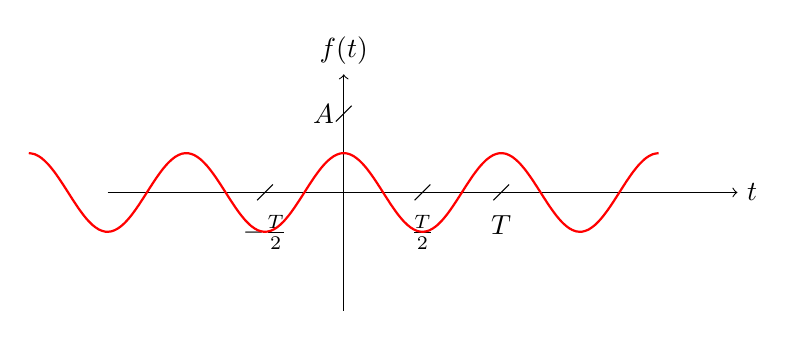
\begin{tikzpicture}
  %\draw (0,0) circle (1in);
  \draw[->] (-3.0,+0.0) -- (+5.0,+0.0) node[right] {$t$};
  \draw[->] (+0.0,-1.5) -- (+0.0,+1.5) node[above] {$f(t)$};
  %\draw[-,red, thick] (-2.5,+0.0) -- (+0.0,+0.0);
  %\draw[-] (-1.0-0.1,-0.1)--(-1.0+0.1,0.1) node[midway, below, outer sep=10pt,align=center] {$-\frac{T}{2}$};
  \draw[-] (-1.0-0.1,-0.1)--(-1.0+0.1,0.1) node[midway, below, outer sep=5pt,align=center] {$-\frac{T}{2}$};
  \draw[-] (+1.0-0.1,-0.1)--(+1.0+0.1,0.1) node[midway, below, outer sep=5pt] {$\frac{T}{2}$};
  \draw[-] (+2.0-0.1,-0.1)--(+2.0+0.1,0.1) node[midway, below, outer sep=5pt] {$T$};
  \draw[-] (-0.1,1.0-0.1)--(+0.1,1.0+0.1) node[midway, left] {$A$};
  
  \draw[scale=1.0,domain=-4:4.0,samples=100,smooth,variable=\x,red,thick] plot ({\x},{0+2.0/4*cos(\x*180.0/3.141592*1*3.141592/1.0)});
  \end{tikzpicture}
\end{figure}

\TT{W przypadku sumowania od $k_{min}=-2$ do $k_{max}=2$ otrzymujemy:}{A partial approximation of the $f(t)$ signal from $k_{min}=-2$ to $k_{max}=2$ results in:}

\begin{figure}[H]
  \centering
  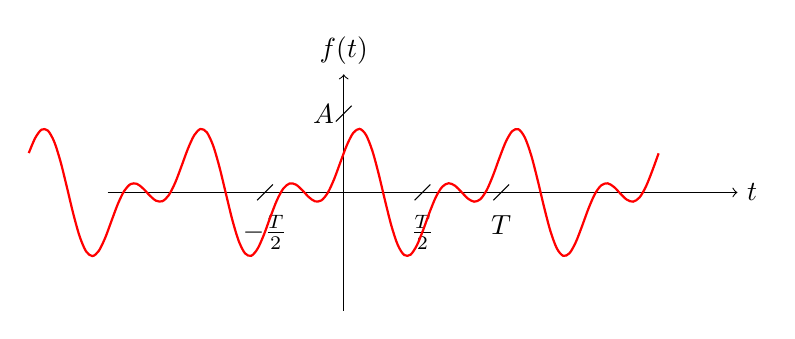
\begin{tikzpicture}
  %\draw (0,0) circle (1in);
  \draw[->] (-3.0,+0.0) -- (+5.0,+0.0) node[right] {$t$};
  \draw[->] (+0.0,-1.5) -- (+0.0,+1.5) node[above] {$f(t)$};
  %\draw[-,red, thick] (-2.5,+0.0) -- (+0.0,+0.0);
  %\draw[-] (-1.0-0.1,-0.1)--(-1.0+0.1,0.1) node[midway, below, outer sep=10pt,align=center] {$-\frac{T}{2}$};
  \draw[-] (-1.0-0.1,-0.1)--(-1.0+0.1,0.1) node[midway, below, outer sep=5pt,align=center] {$-\frac{T}{2}$};
  \draw[-] (+1.0-0.1,-0.1)--(+1.0+0.1,0.1) node[midway, below, outer sep=5pt] {$\frac{T}{2}$};
  \draw[-] (+2.0-0.1,-0.1)--(+2.0+0.1,0.1) node[midway, below, outer sep=5pt] {$T$};
  \draw[-] (-0.1,1.0-0.1)--(+0.1,1.0+0.1) node[midway, left] {$A$};
  
  \draw[scale=1.0,domain=-4:4.0,samples=100,smooth,variable=\x,red,thick] plot ({\x},{0.0+2.0/4*cos(\x*180.0/3.141592*1*3.141592/1.0)+4.0/(3*3.141592)*sin(\x*180.0/3.141592*2*3.141592/1.0)});
  \end{tikzpicture}
\end{figure}

\TT{W przypadku sumowania od $k_{min}=-4$ do $k_{max}=4$ otrzymujemy:}{A partial approximation of the $f(t)$ signal from $k_{min}=-4$ to $k_{max}=4$ results in:}

\begin{figure}[H]
  \centering
  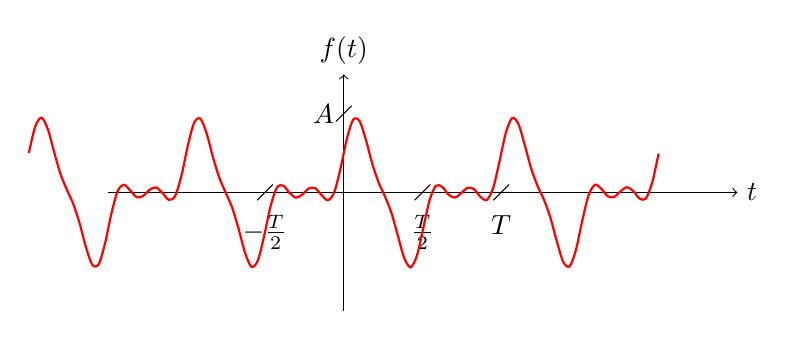
\begin{tikzpicture}
  %\draw (0,0) circle (1in);
  \draw[->] (-3.0,+0.0) -- (+5.0,+0.0) node[right] {$t$};
  \draw[->] (+0.0,-1.5) -- (+0.0,+1.5) node[above] {$f(t)$};
  %\draw[-,red, thick] (-2.5,+0.0) -- (+0.0,+0.0);
  %\draw[-] (-1.0-0.1,-0.1)--(-1.0+0.1,0.1) node[midway, below, outer sep=10pt,align=center] {$-\frac{T}{2}$};
  \draw[-] (-1.0-0.1,-0.1)--(-1.0+0.1,0.1) node[midway, below, outer sep=5pt,align=center] {$-\frac{T}{2}$};
  \draw[-] (+1.0-0.1,-0.1)--(+1.0+0.1,0.1) node[midway, below, outer sep=5pt] {$\frac{T}{2}$};
  \draw[-] (+2.0-0.1,-0.1)--(+2.0+0.1,0.1) node[midway, below, outer sep=5pt] {$T$};
  \draw[-] (-0.1,1.0-0.1)--(+0.1,1.0+0.1) node[midway, left] {$A$};
  
  \draw[scale=1.0,domain=-4:4.0,samples=100,smooth,variable=\x,red,thick] plot ({\x},{0.0+2.0/4*cos(\x*180.0/3.141592*1*3.141592/1.0)+4.0/(3*3.141592)*sin(\x*180.0/3.141592*2*3.141592/1.0)+8.0/(15*3.141592)*sin(\x*180.0/3.141592*4*3.141592/1.0)});
  \end{tikzpicture}
\end{figure}

\TT{W przypadku sumowania od $k_{min}=-10$ do $k_{max}=10$ otrzymujemy:}{A partial approximation of the $f(t)$ signal from $k_{min}=-10$ to $k_{max}=10$ results in:} 

\begin{figure}[H]
  \centering
  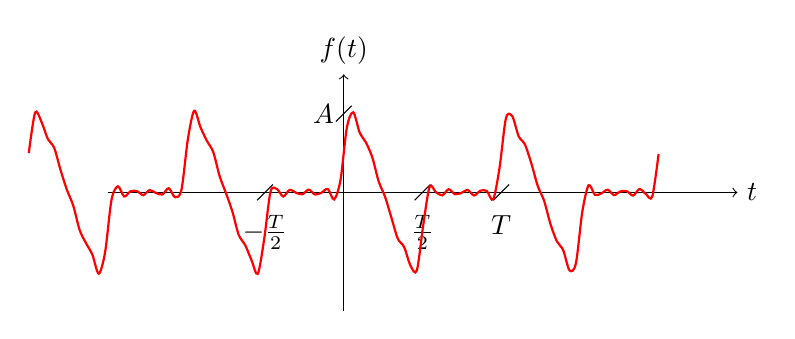
\begin{tikzpicture}
  %\draw (0,0) circle (1in);
  \draw[->] (-3.0,+0.0) -- (+5.0,+0.0) node[right] {$t$};
  \draw[->] (+0.0,-1.5) -- (+0.0,+1.5) node[above] {$f(t)$};
  %\draw[-,red, thick] (-2.5,+0.0) -- (+0.0,+0.0);
  %\draw[-] (-1.0-0.1,-0.1)--(-1.0+0.1,0.1) node[midway, below, outer sep=10pt,align=center] {$-\frac{T}{2}$};
  \draw[-] (-1.0-0.1,-0.1)--(-1.0+0.1,0.1) node[midway, below, outer sep=5pt,align=center] {$-\frac{T}{2}$};
  \draw[-] (+1.0-0.1,-0.1)--(+1.0+0.1,0.1) node[midway, below, outer sep=5pt] {$\frac{T}{2}$};
  \draw[-] (+2.0-0.1,-0.1)--(+2.0+0.1,0.1) node[midway, below, outer sep=5pt] {$T$};
  \draw[-] (-0.1,1.0-0.1)--(+0.1,1.0+0.1) node[midway, left] {$A$};
  
  \draw[scale=1.0,domain=-4:4.0,samples=100,smooth,variable=\x,red,thick] plot ({\x},{0.0+2.0/4*cos(\x*180.0/3.141592*1*3.141592/1.0)+4.0/(3*3.141592)*sin(\x*180.0/3.141592*2*3.141592/1.0)+8.0/(15*3.141592)*sin(\x*180.0/3.141592*4*3.141592/1.0)+12.0/(35*3.141592)*sin(\x*180.0/3.141592*6*3.141592/1.0)+16.0/(63*3.141592)*sin(\x*180.0/3.141592*8*3.141592/1.0)});
  \end{tikzpicture}
\end{figure}

\TT{W przypadku sumowania od $k_{min}=-20$ do $k_{max}=20$ otrzymujemy:}{A partial approximation of the $f(t)$ signal from $k_{min}=-20$ to $k_{max}=20$ results in:} 

\begin{figure}[H]
  \centering
  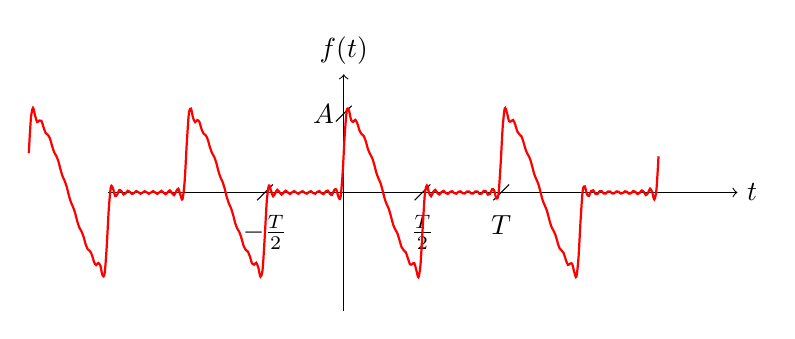
\begin{tikzpicture}
  %\draw (0,0) circle (1in);
  \draw[->] (-3.0,+0.0) -- (+5.0,+0.0) node[right] {$t$};
  \draw[->] (+0.0,-1.5) -- (+0.0,+1.5) node[above] {$f(t)$};
  %\draw[-,red, thick] (-2.5,+0.0) -- (+0.0,+0.0);
  %\draw[-] (-1.0-0.1,-0.1)--(-1.0+0.1,0.1) node[midway, below, outer sep=10pt,align=center] {$-\frac{T}{2}$};
  \draw[-] (-1.0-0.1,-0.1)--(-1.0+0.1,0.1) node[midway, below, outer sep=5pt,align=center] {$-\frac{T}{2}$};
  \draw[-] (+1.0-0.1,-0.1)--(+1.0+0.1,0.1) node[midway, below, outer sep=5pt] {$\frac{T}{2}$};
  \draw[-] (+2.0-0.1,-0.1)--(+2.0+0.1,0.1) node[midway, below, outer sep=5pt] {$T$};
  \draw[-] (-0.1,1.0-0.1)--(+0.1,1.0+0.1) node[midway, left] {$A$};
  
  \draw[scale=1.0,domain=-4:4.0,samples=300,smooth,variable=\x,red,thick] plot ({\x},{0.0+2.0/4*cos(\x*180.0/3.141592*1*3.141592/1.0)+4.0/(3*3.141592)*sin(\x*180.0/3.141592*2*3.141592/1.0)+8.0/(15*3.141592)*sin(\x*180.0/3.141592*4*3.141592/1.0)+12.0/(35*3.141592)*sin(\x*180.0/3.141592*6*3.141592/1.0)+16.0/(63*3.141592)*sin(\x*180.0/3.141592*8*3.141592/1.0)+20.0/(99*3.141592)*sin(\x*180.0/3.141592*10*3.141592/1.0)+24.0/(143*3.141592)*sin(\x*180.0/3.141592*12*3.141592/1.0)+28.0/(195*3.141592)*sin(\x*180.0/3.141592*14*3.141592/1.0)+32.0/(255*3.141592)*sin(\x*180.0/3.141592*16*3.141592/1.0)+36.0/(323*3.141592)*sin(\x*180.0/3.141592*18*3.141592/1.0)});
  \end{tikzpicture}
\end{figure}

\TT{W granicy sumowania od $k_{min}=-\infty$ do $k_{max}=\infty$ otrzymujemy oryginalny sygnał.}{Approximation of the $f(t)$ signal for from $k_{min}=-\infty$ to $k_{max}=\infty$ results in oryginal signal.}

\end{task}